% solution_1.tex
% by Troy Hix, April 2005
%----------------------------------------------------------------------------
\begin{figure}
\centering
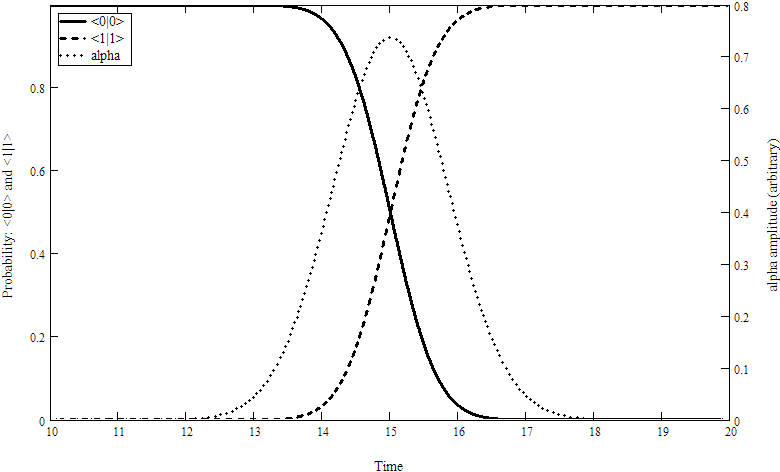
\includegraphics[width=5.00in]
{solution_1/solution_1.png}\\
\caption[Single color optimal solution]{Single color optimal solution. With $\sigma_{\alpha}\equiv 2$, this local optimum occurs when $A=0.737832313319$. Many more local optima occur with increasing $A$. If the pulse area is $\xi$, then $\xi - \pi/2 \sim 10^{-12}$ (the precision of $A$). In the literature, this is called a $\pi$--pulse.}
\label{solution one}
\end{figure} 
%----------------------------------------------------------------------------
